% !TeX root = ../thuthesis-example.tex

\chapter{测试驱动开发的设计与实现}
\label{chap:tdd}

测试驱动开发(Test-Driven Development, TDD)是一种软件开发方法论,核心在于先编写测试代码再实现功能代码。这种"测试先行"范式要求开发者首先明确定义预期行为与结果,随后实现满足测试条件的功能代码。TDD遵循"红-绿-重构"循环:编写一个失败的测试(红),实现最小可行代码使测试通过(绿),最后改进代码结构与设计(重构)。

bolt.SE的测试模块是对TDD理念的工程化实现,使开发者能创建、管理测试用例,并引导大语言模型(LLM)生成满足这些测试要求的代码。本章分析TDD概念、方法论价值及bolt.SE的测试功能技术实现。

\section{测试驱动开发对bolt.SE的意义}

在大型语言模型驱动的软件开发中,测试驱动方法具有特殊价值。测试用例为LLM提供结构化需求表达,降低需求理解的歧义性,实现需求形式化。通过明确定义预期行为,测试还为LLM提供具体目标,有效限定代码生成的解空间。严格的测试约束能够降低LLM生成错误或不切实际代码的风险,确保输出符合验证逻辑的结果。测试机制提供客观验证标准,保证LLM生成的代码不仅表面合理,更能正确运行。同时,测试结果为LLM提供结构化反馈,引导其精确改进代码缺陷,促进代码质量的持续优化。

此外,TDD在传统软件工程中的优势同样适用于LLM驱动开发:促进模块化设计、提供快速反馈、形成活文档并聚焦实现目标。bolt.SE将测试代码集成至对话上下文,实现了LLM与测试用例的协同工作模式,既保留了LLM的生成灵活性,又引入了软件工程的严谨验证机制。

\section{bolt.SE中的Jest测试框架应用}

bolt.SE选择Jest作为核心测试框架,主要看中其在前端开发生态中的主流地位。由Facebook开发的Jest提供了零配置的快速部署体验,开发者只需安装依赖即可开始编写测试,无需繁琐的环境配置\cite{Jest2023}。其声明式API使测试代码结构清晰,易于LLM理解和生成,而丰富的断言器与快照测试功能则为各类应用场景提供了验证支持。

Jest测试在bolt.SE中采用直观的结构组织:通过\texttt{describe}块定义测试套件,用\texttt{test}/\texttt{it}函数声明测试用例,并使用\texttt{expect}配合各类匹配器表达验证条件,如下所示:

\begin{minted}{javascript}
describe('Calculator', () => {
  test('adds 1 + 2 to equal 3', () => {
    expect(add(1, 2)).toBe(3);
  });
  
  test('subtracts 5 - 2 to equal 3', () => {
    expect(subtract(5, 2)).toBe(3);
  });
});
\end{minted}

bolt.SE测试模块能解析此结构,提取测试套件和用例的层次关系,构建测试树模型。系统将测试信息转换为LLM可理解的约束条件,在对话启动时注入上下文,引导模型生成符合测试要求的代码。这种测试驱动的开发工作流程形成完整循环:从测试定义、结构提取、上下文注入,到代码生成、验证与迭代优化,有效融合了TDD方法论与AI辅助开发的优势。

\section{bolt.SE中的测试功能实现}

图\ref{fig:test_sequence}展示了测试功能的完整流程,包括用户测试定义、使用及验证的完整流程与跨组件信息传递机制。

\begin{figure}[H]
  \centering
  \makebox[\textwidth][c]{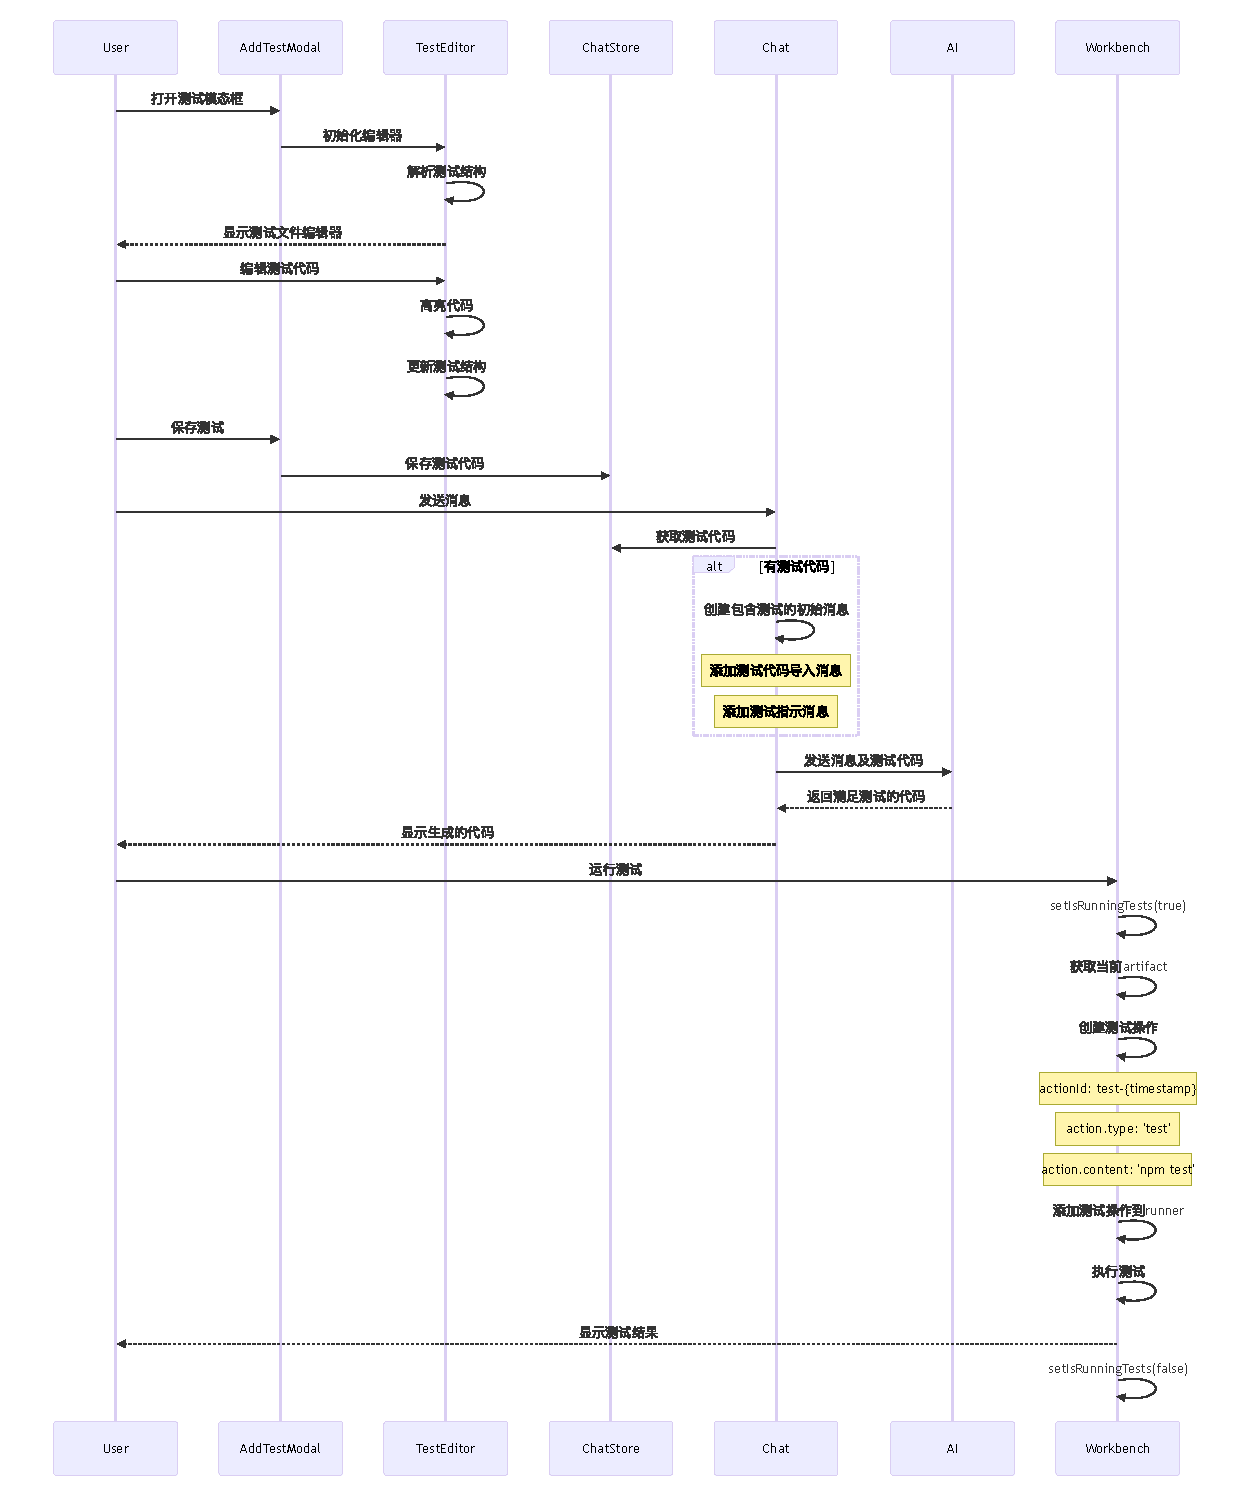
\includegraphics[width=1.2\textwidth]{figures/bolt_test_sequence.pdf}}
  \caption{测试功能流程图:展示用户测试定义、使用及验证的完整流程与跨组件信息传递机制}
  \label{fig:test_sequence}
\end{figure}

bolt.SE测试系统系统基于正则表达式精确解析\texttt{describe}和\texttt{it}/\texttt{test}函数调用,构建结构化测试表示。此解析机制将非结构化测试代码转换为层次化数据模型,为后续操作提供基础。测试界面实现了导航机制,通过树形结构展示测试组织,并支持测试项与代码区域的精确定位与高亮显示,降低认知负荷。测试代码在系统启动时被转换为形式化约束条件,通过结构化描述明确功能预期,提供精确的功能边界定义。这种方法显著减少了需求的歧义性,使代码能够直接针对具体测试条件进行验证。系统还包含环境配置自动化能力,自动添加必要依赖和测试脚本,确保测试环境一致性。当执行测试失败时,系统将错误信息结构化并转换为具体修复指导,形成完整的反馈闭环,驱动代码迭代优化。

bolt.SE测试系统采用组件化架构,主要包含以下核心模块:

\begin{itemize}
  \item 用户界面层:
    \begin{itemize}
      \item \texttt{AddTestModal}:测试管理的主入口,支持测试创建与编辑
      \item \texttt{TestEditor}:代码编辑器组件,提供语法高亮与结构可视化
      \item \texttt{TestStructure}:测试树渲染组件,展示测试套件与用例的层次关系
    \end{itemize}
  
  \item 数据处理层:
    \begin{itemize}
      \item \texttt{chatStore}:管理当前会话的测试代码集合
      \item \texttt{IndexedDB}:持久化存储测试定义,支持跨会话访问
    \end{itemize}
  
  \item 测试执行层:
    \begin{itemize}
      \item \texttt{Workbench}:提供测试运行环境与命令执行
      \item \texttt{ActionRunner}:负责测试调度与结果采集
    \end{itemize}
  
  \item AI交互层:处理测试代码与LLM的信息交换与指令生成
\end{itemize}

bolt.SE定义了结构化的测试数据模型,如图\ref{fig:test_class}所示:

\begin{figure}[H]
  \centering
  \makebox[\textwidth][c]{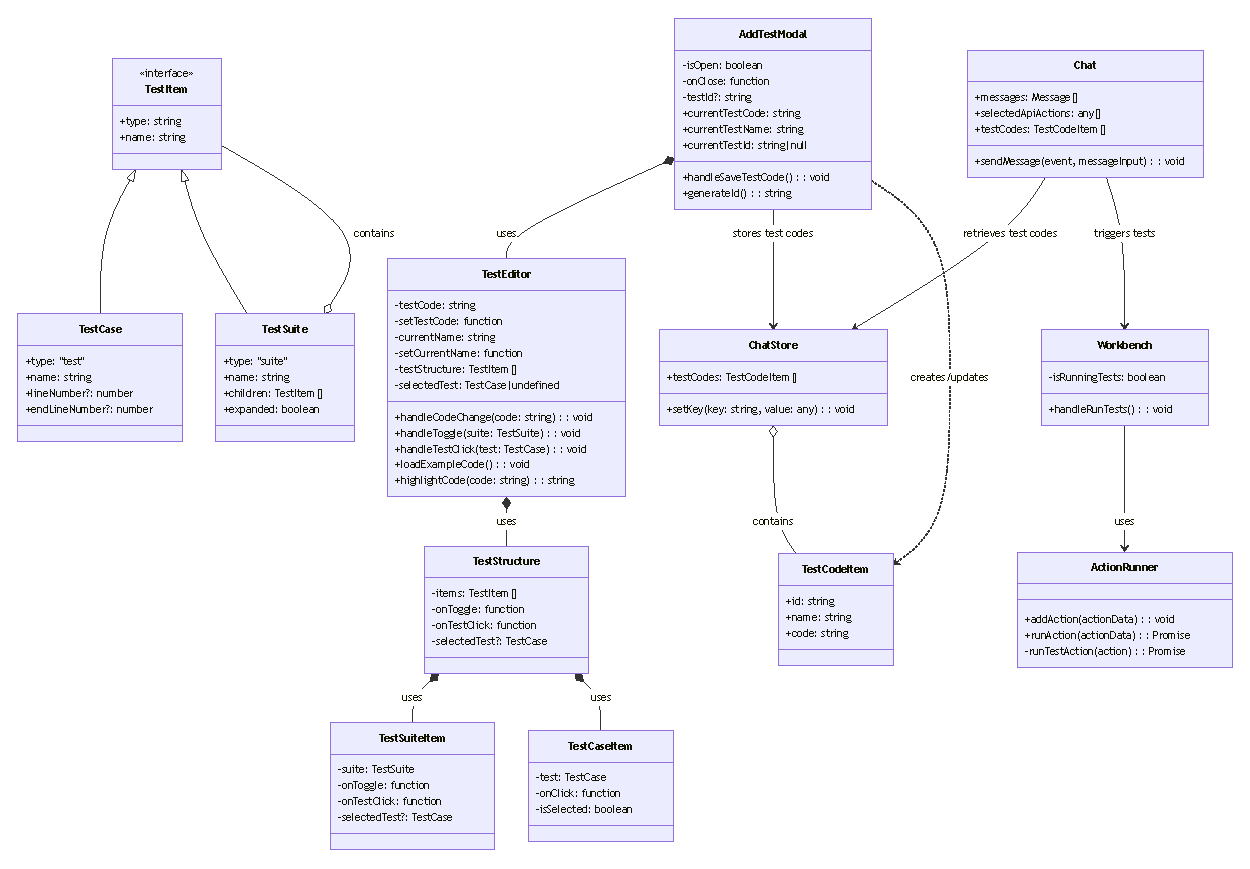
\includegraphics[width=1.3\textwidth]{figures/bolt_test_class.pdf}}
  \caption{测试数据模型类图:描述测试定义的核心数据结构及关系,包含测试代码项、测试用例与测试套件的层次组织}
  \label{fig:test_class}
\end{figure}

测试系统的核心数据结构包括:

\begin{itemize}
  \item TestCodeItem:测试文件实体,包含唯一标识符、名称与代码内容。
  
  \item TestItem:测试项基础接口,定义共用的类型与名称属性。
  
  \item TestCase:具体测试用例,标识类型为"test",记录代码位置信息。
  
  \item TestSuite:测试套件,标识类型为"suite",包含子测试项集合与展开状态。
\end{itemize}

\section{实例应用场景}
\label{sec:tdd-example}

本节通过JavaScript计算器的完整开发流程,展示bolt.SE中基于"红–绿–重构"循环的测试驱动开发过程及LLM参与的自动修复机制。

在测试驱动开发的起始阶段,开发者首先通过AddTestModal组件创建测试代码,如图\ref{fig:tdd_add_test}所示,系统解析测试结构并以树形展示,确定开发任务范围:

\begin{figure}[H]
  \centering
  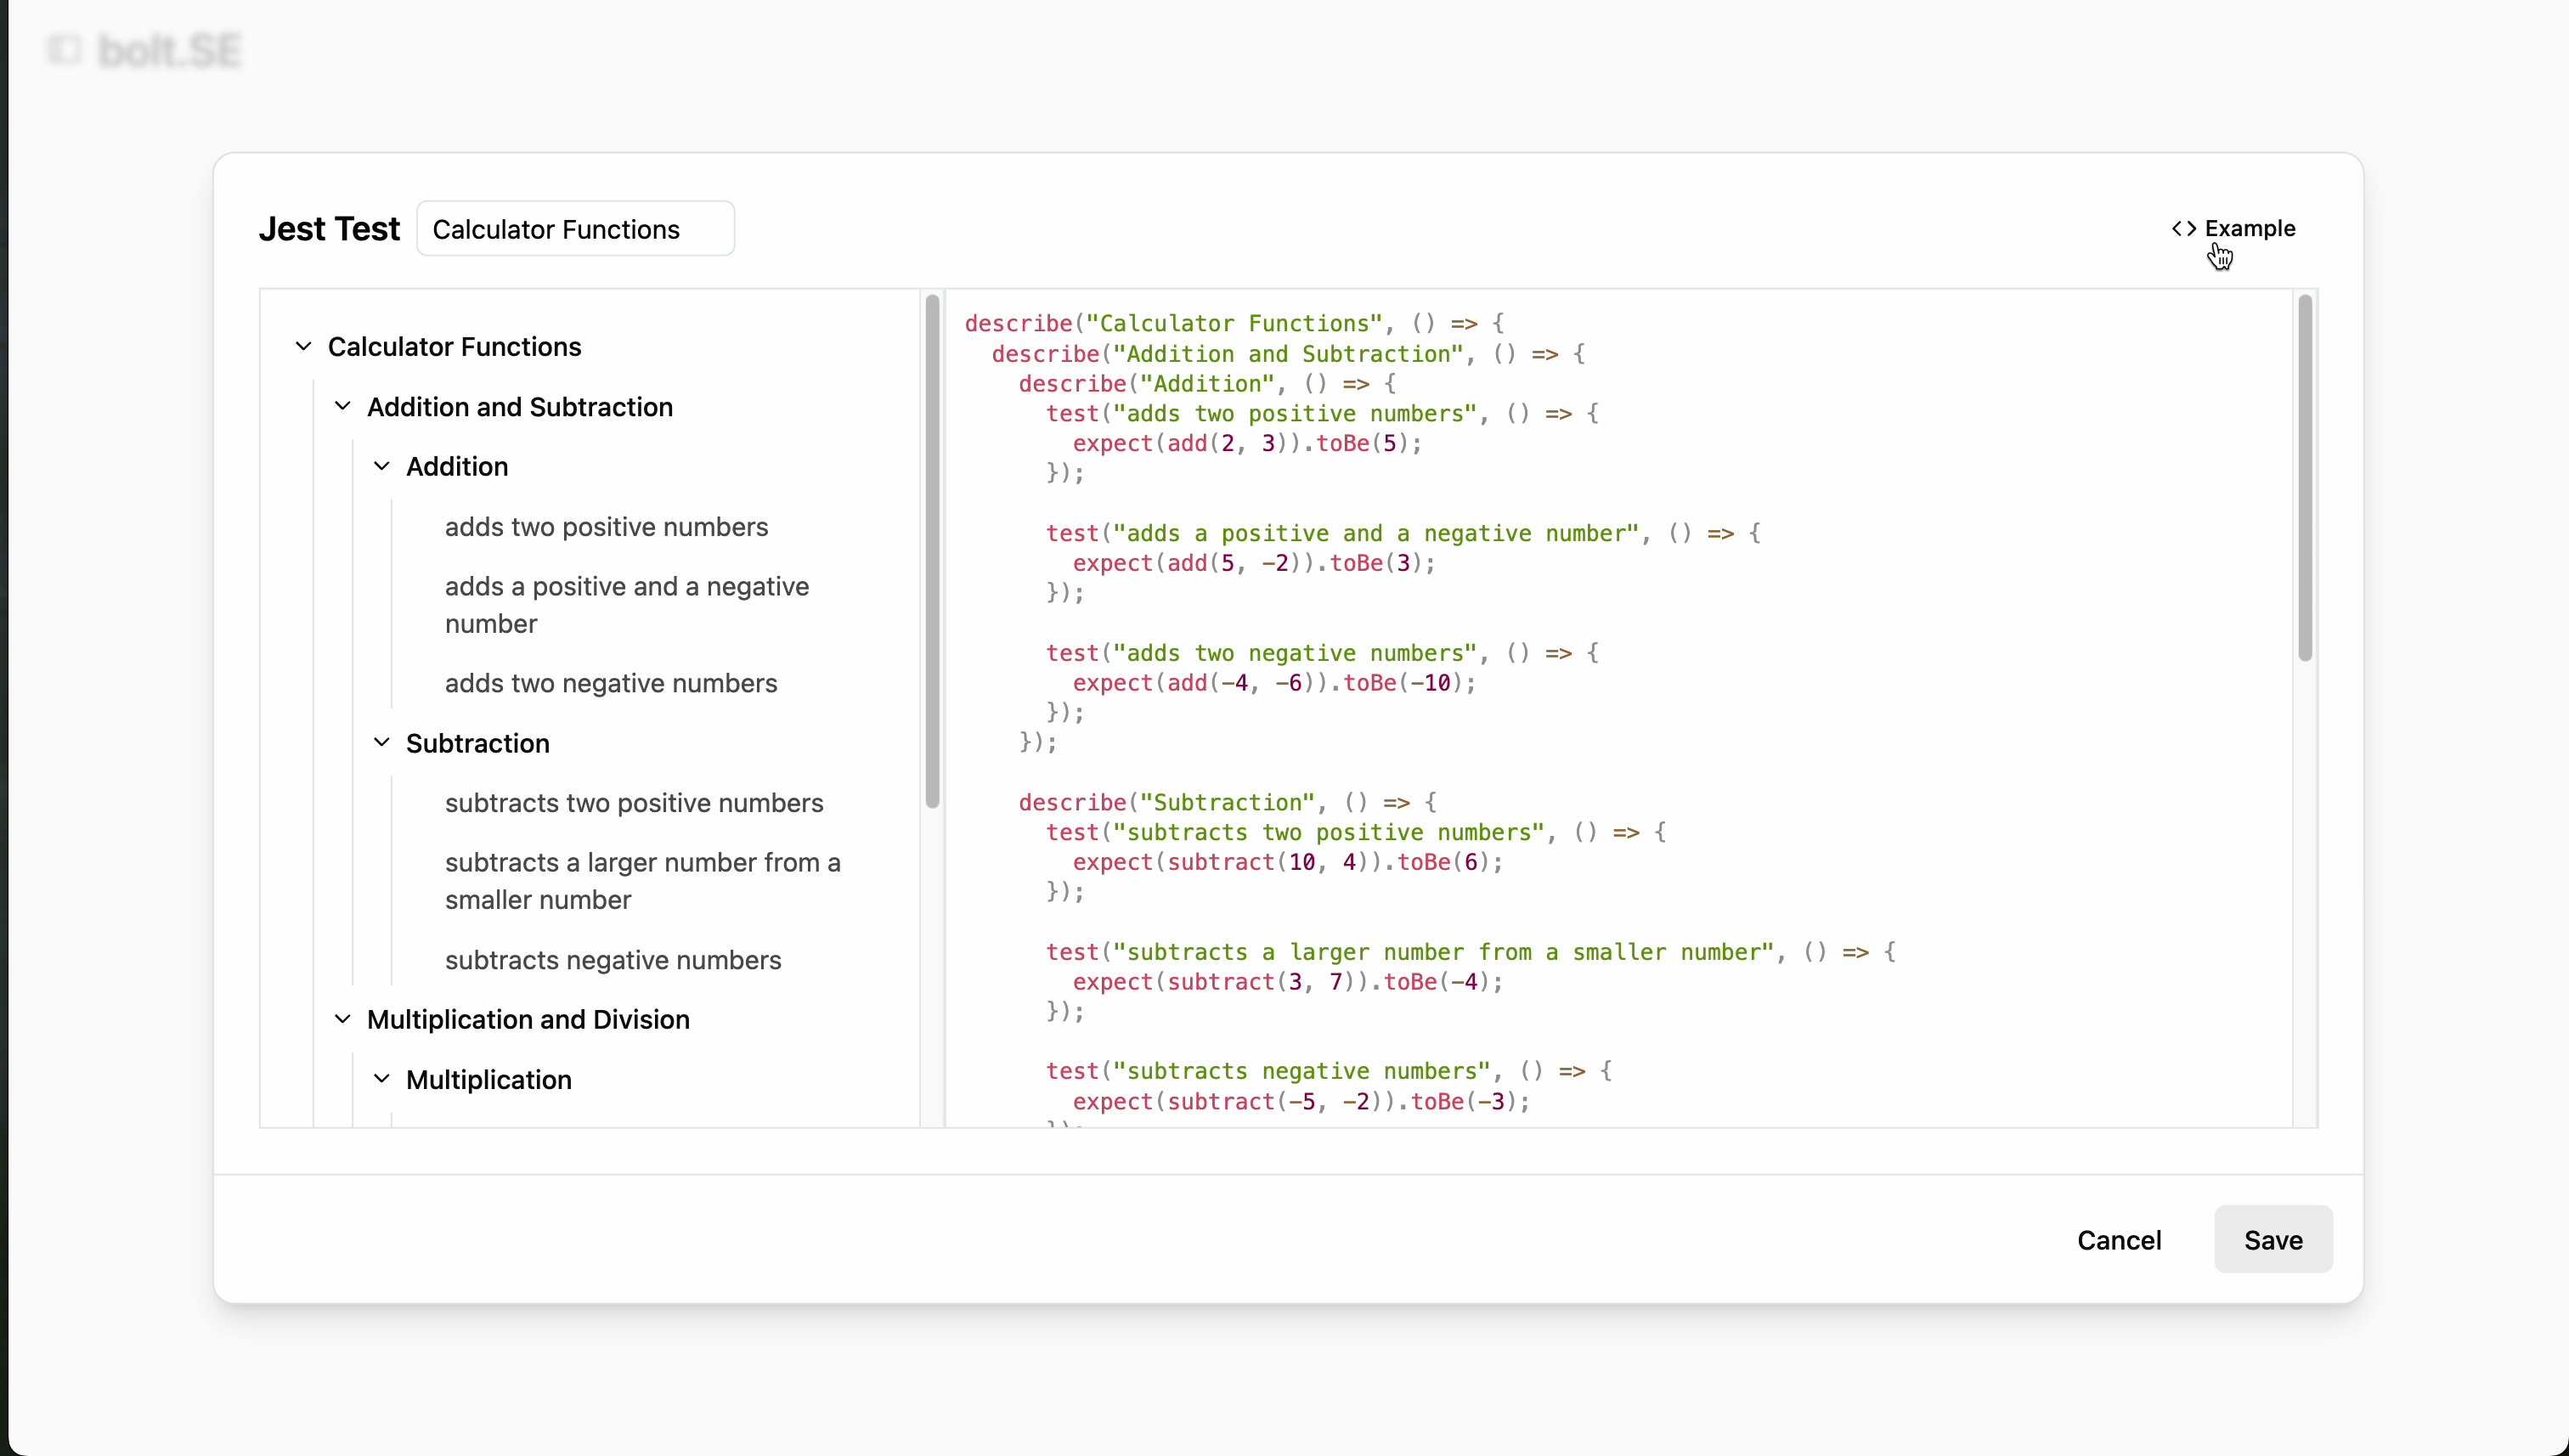
\includegraphics[width=.9\textwidth]{figures/screenshots/tdd/add_test_modal.png}
  \caption{在AddTestModal中粘贴\texttt{calculator\_functions.test.js},系统解析出\textit{Calculator Functions}测试套件与12条断言,并以树形结构展示}
  \label{fig:tdd_add_test}
\end{figure}

开发者随后在聊天窗口输入自然语言描述需求:\texttt{Build a calculator},系统自动注入测试文件与指导语,为LLM提供明确功能规格,如图\ref{fig:tdd_prompt}所示:

\begin{figure}[H]
  \centering
  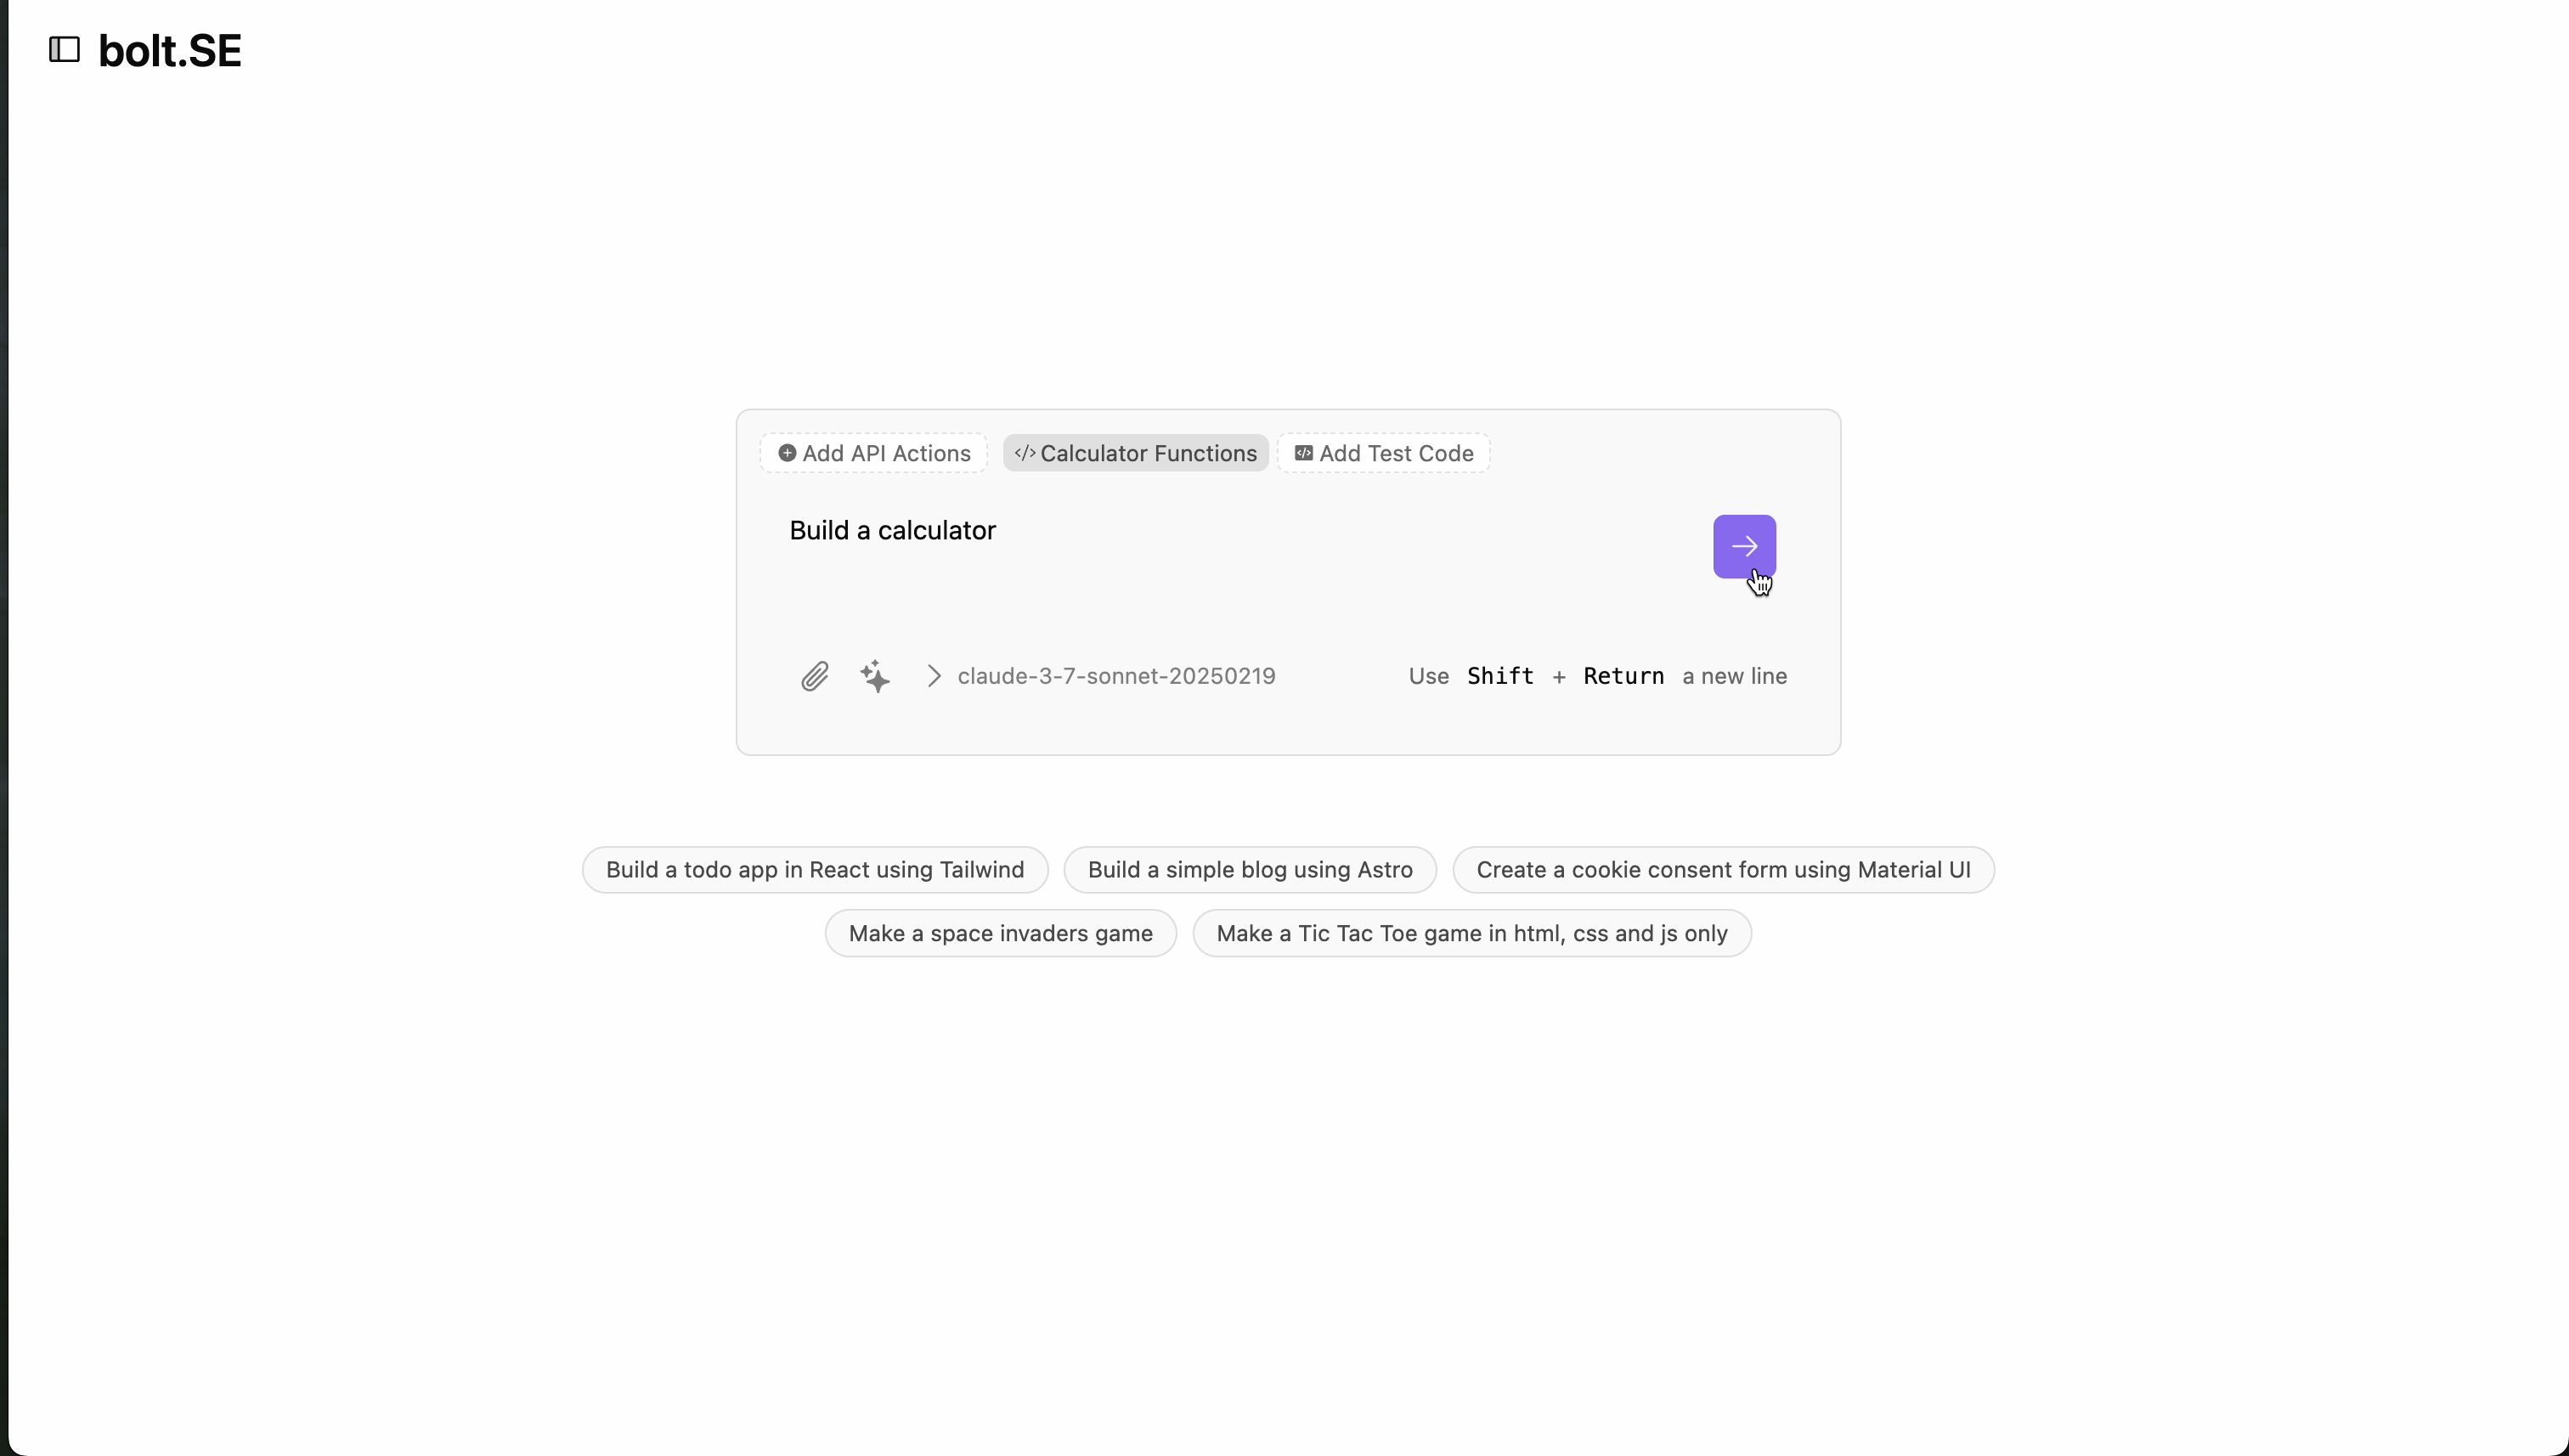
\includegraphics[width=.9\textwidth]{figures/screenshots/tdd/calculator_prompt.png}
  \caption{开发者在聊天窗口输入\texttt{Build a calculator}的需求,系统自动注入测试文件与指导语,为LLM提供明确功能规格}
  \label{fig:tdd_prompt}
\end{figure}

完成测试定义后,LLM分析测试规格并生成相应实现,包括四个算术函数与测试配置。测试执行结果显示全部通过(图\ref{fig:tdd_green_initial}),表明当前实现符合测试规格要求:

\begin{figure}[H]
  \centering
  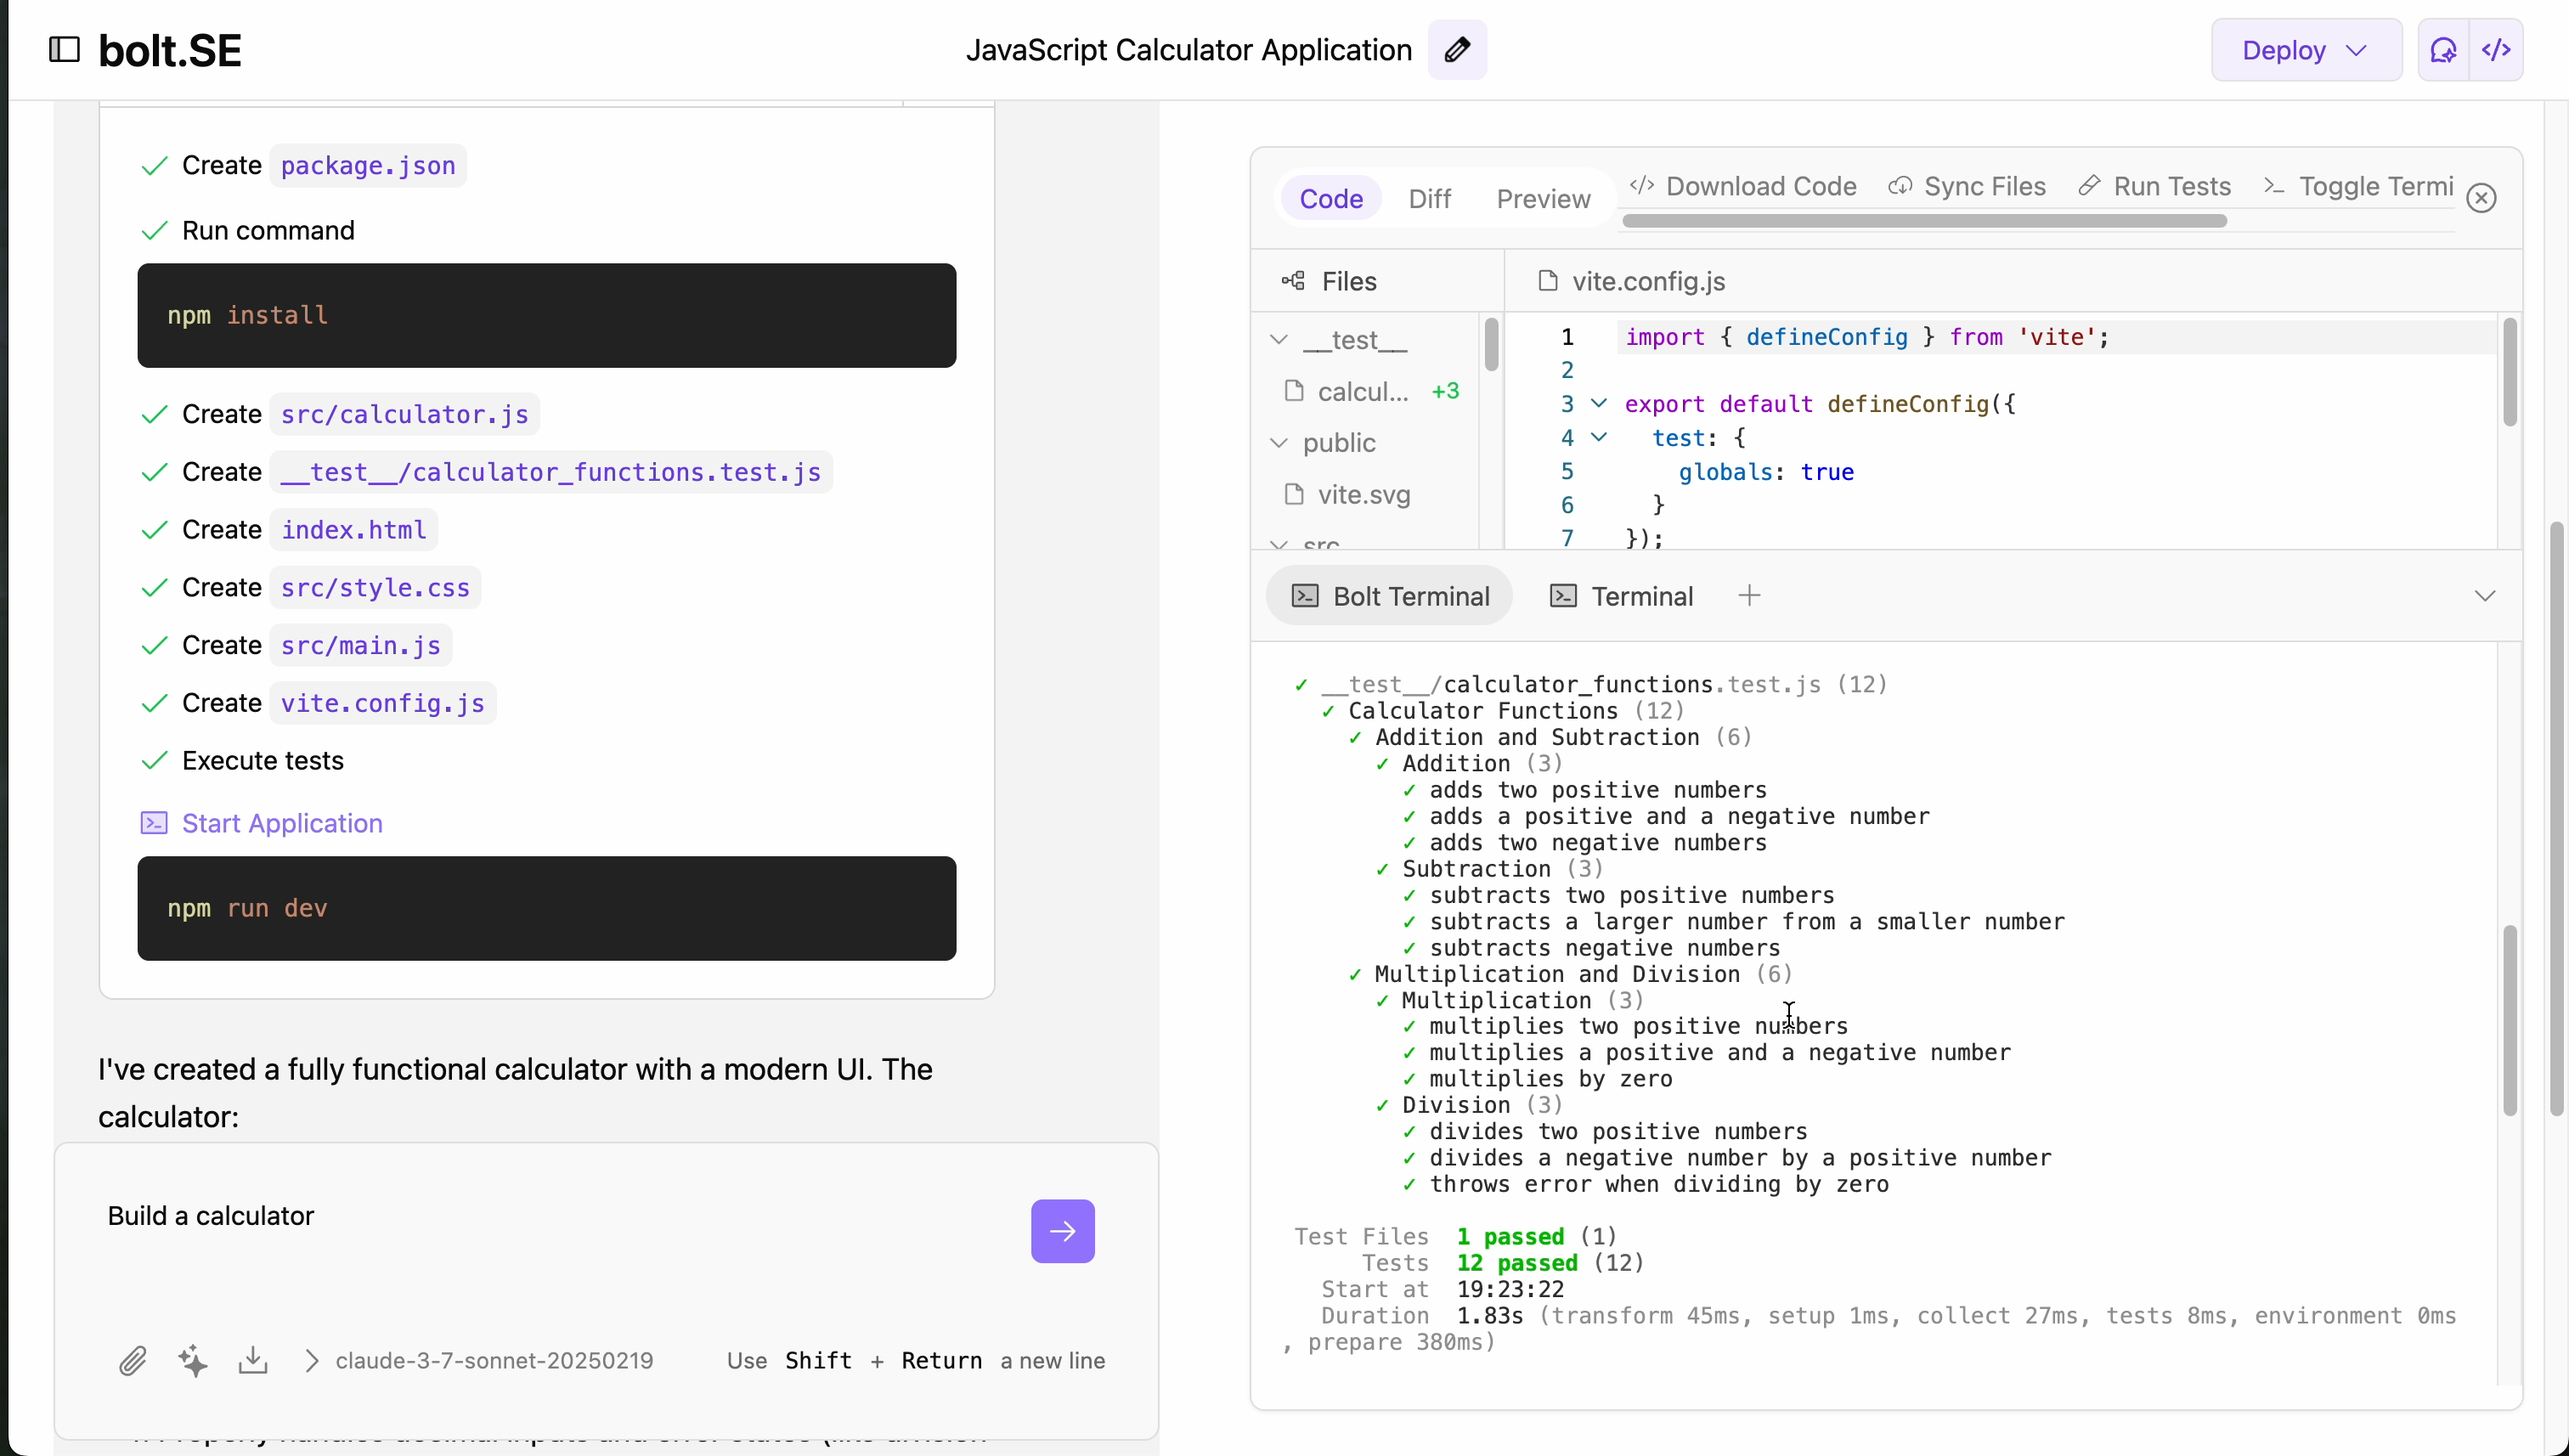
\includegraphics[width=.9\textwidth]{figures/screenshots/tdd/green_pass_initial.png}
  \caption{LLM基于测试用例生成实现代码,运行测试后显示12条断言全部通过}
  \label{fig:tdd_green_initial}
\end{figure}

为演示迭代修复流程,开发者修改一条加法测试断言为\verb|expect(add(2, 3)).toBe(0);|,相当于引入“2+3应等于0”的特殊要求。执行测试后,系统进入红灯阶段(图\ref{fig:tdd_red}):

\begin{figure}[H]
  \centering
  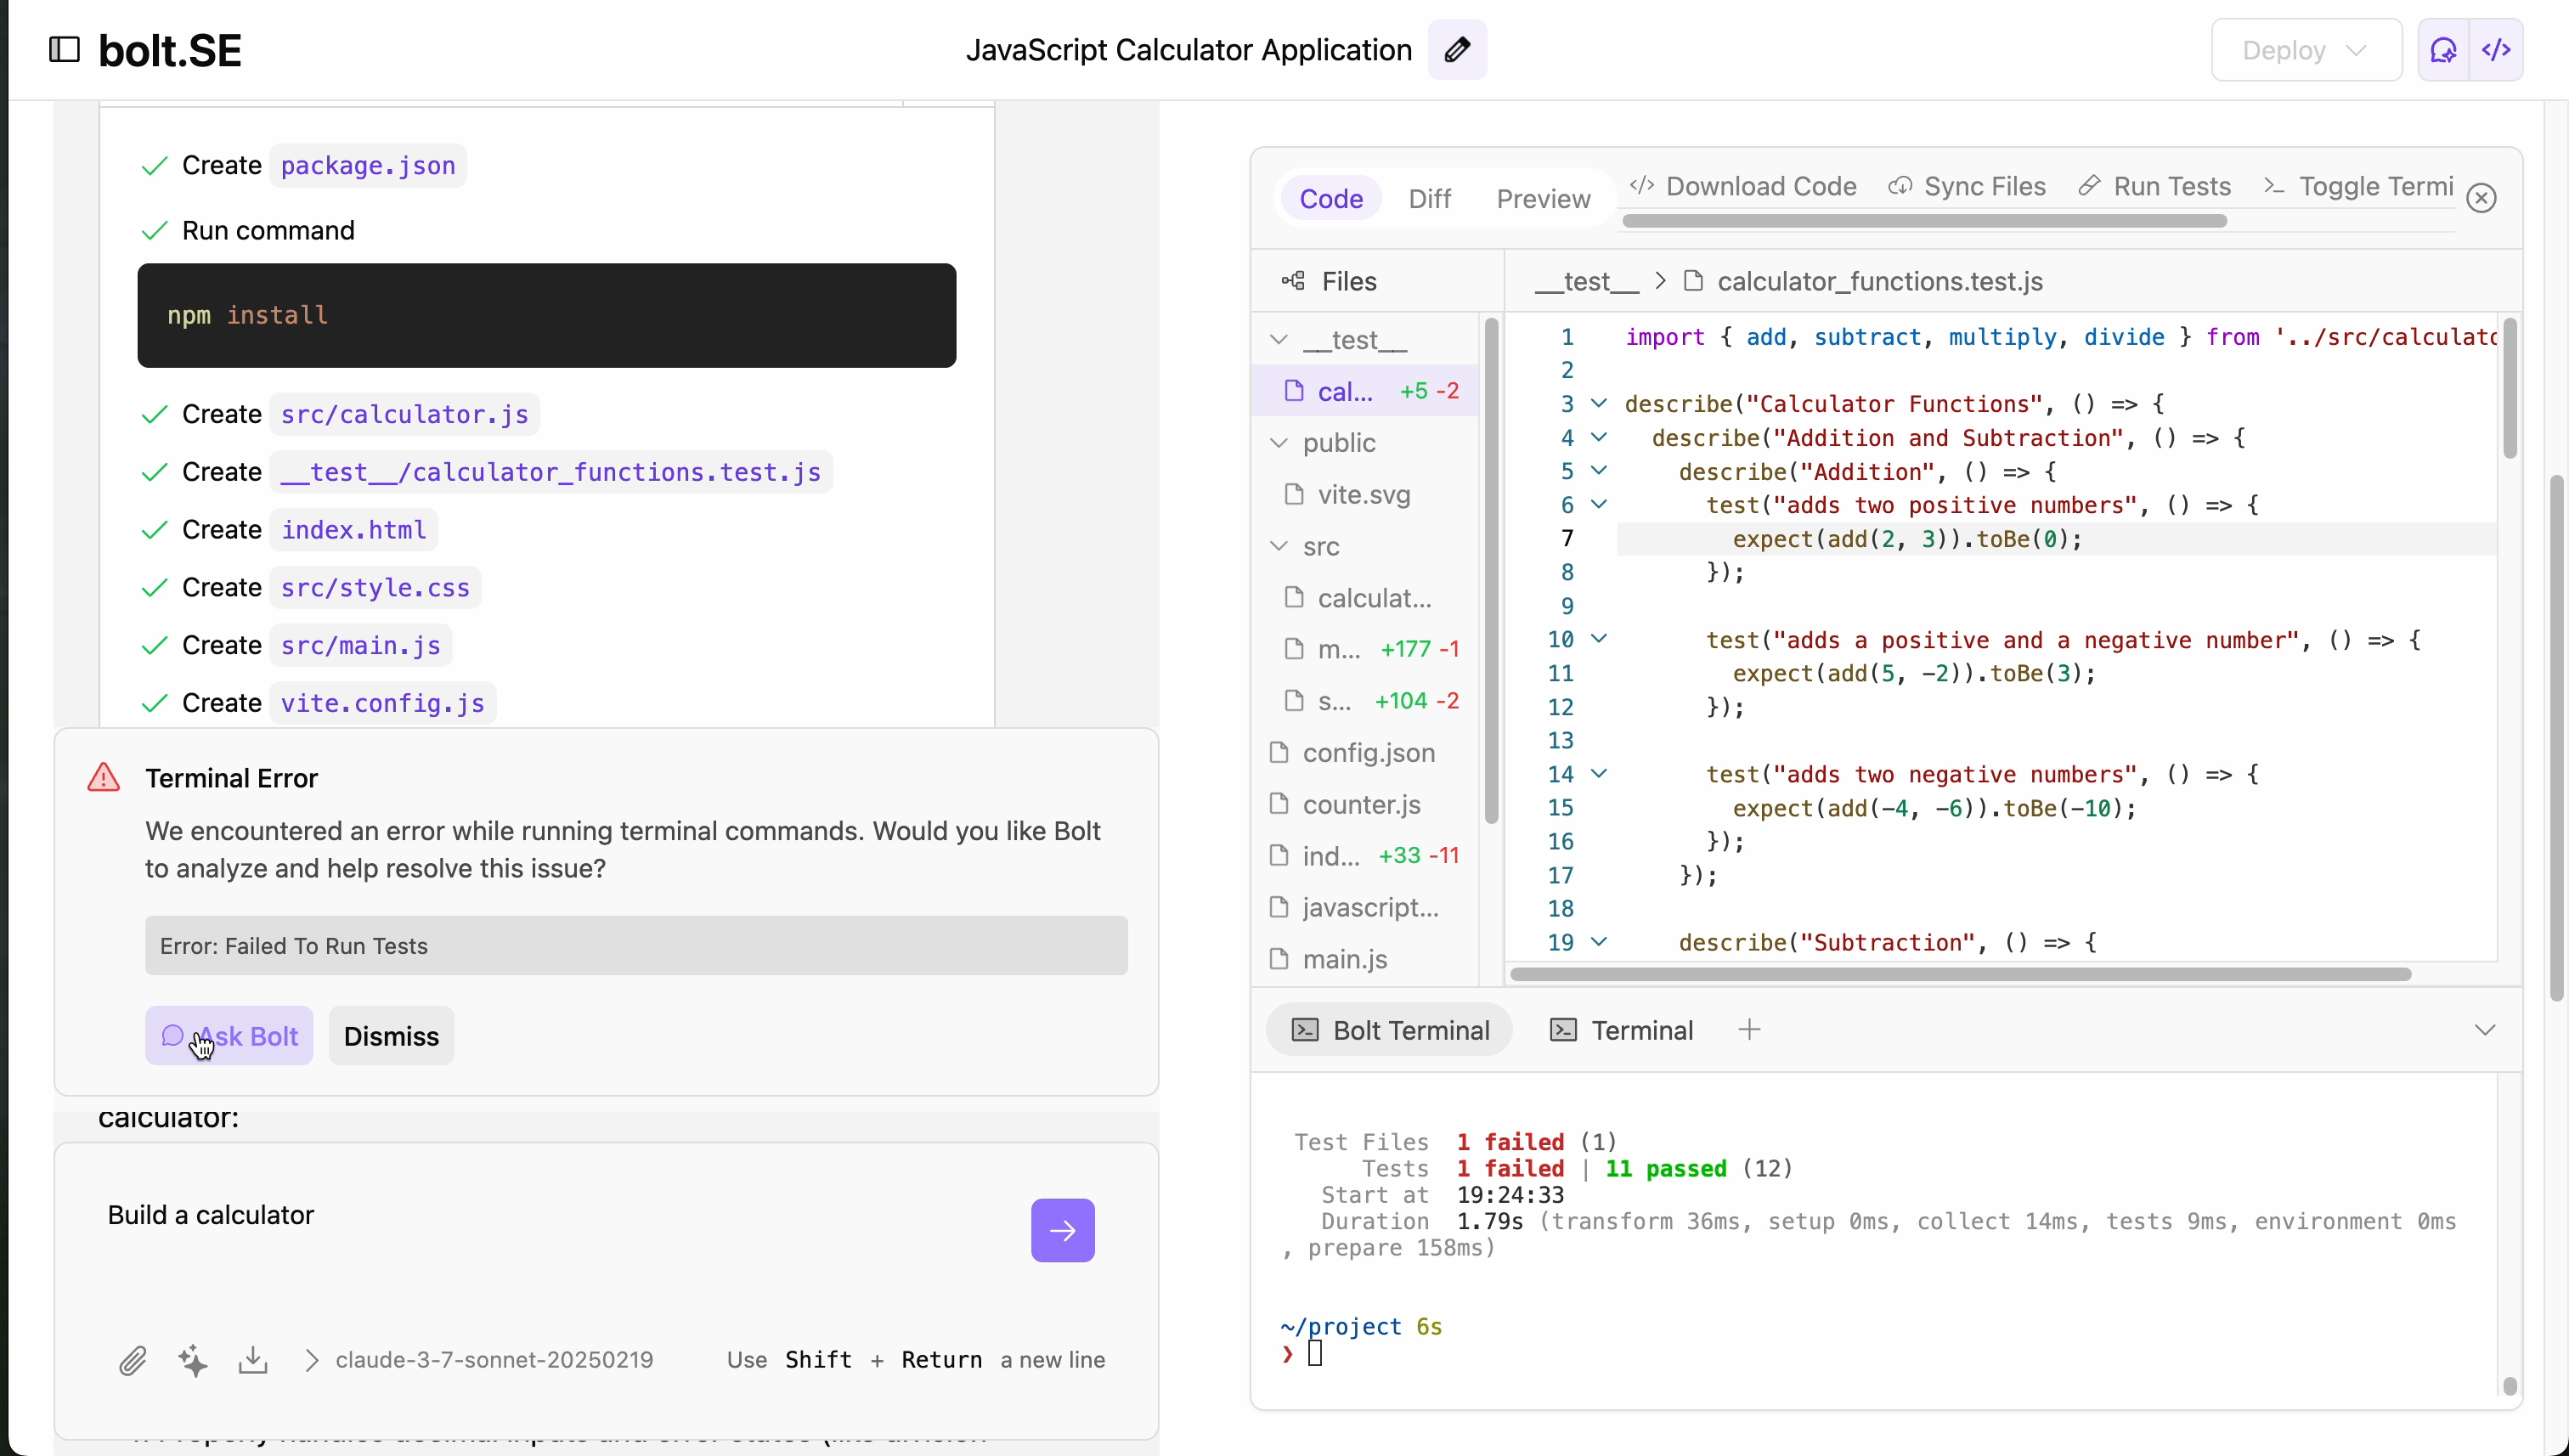
\includegraphics[width=.9\textwidth]{figures/screenshots/tdd/test_edit_fail.png}
  \caption{修改测试断言后执行测试,出现一条失败记录,系统进入红灯阶段}
  \label{fig:tdd_red}
\end{figure}

系统将测试失败信息传递给LLM,模型识别出需要对特定输入做特殊处理,并生成相应补丁代码(图\ref{fig:tdd_fix}):

\begin{figure}[H]
  \centering
  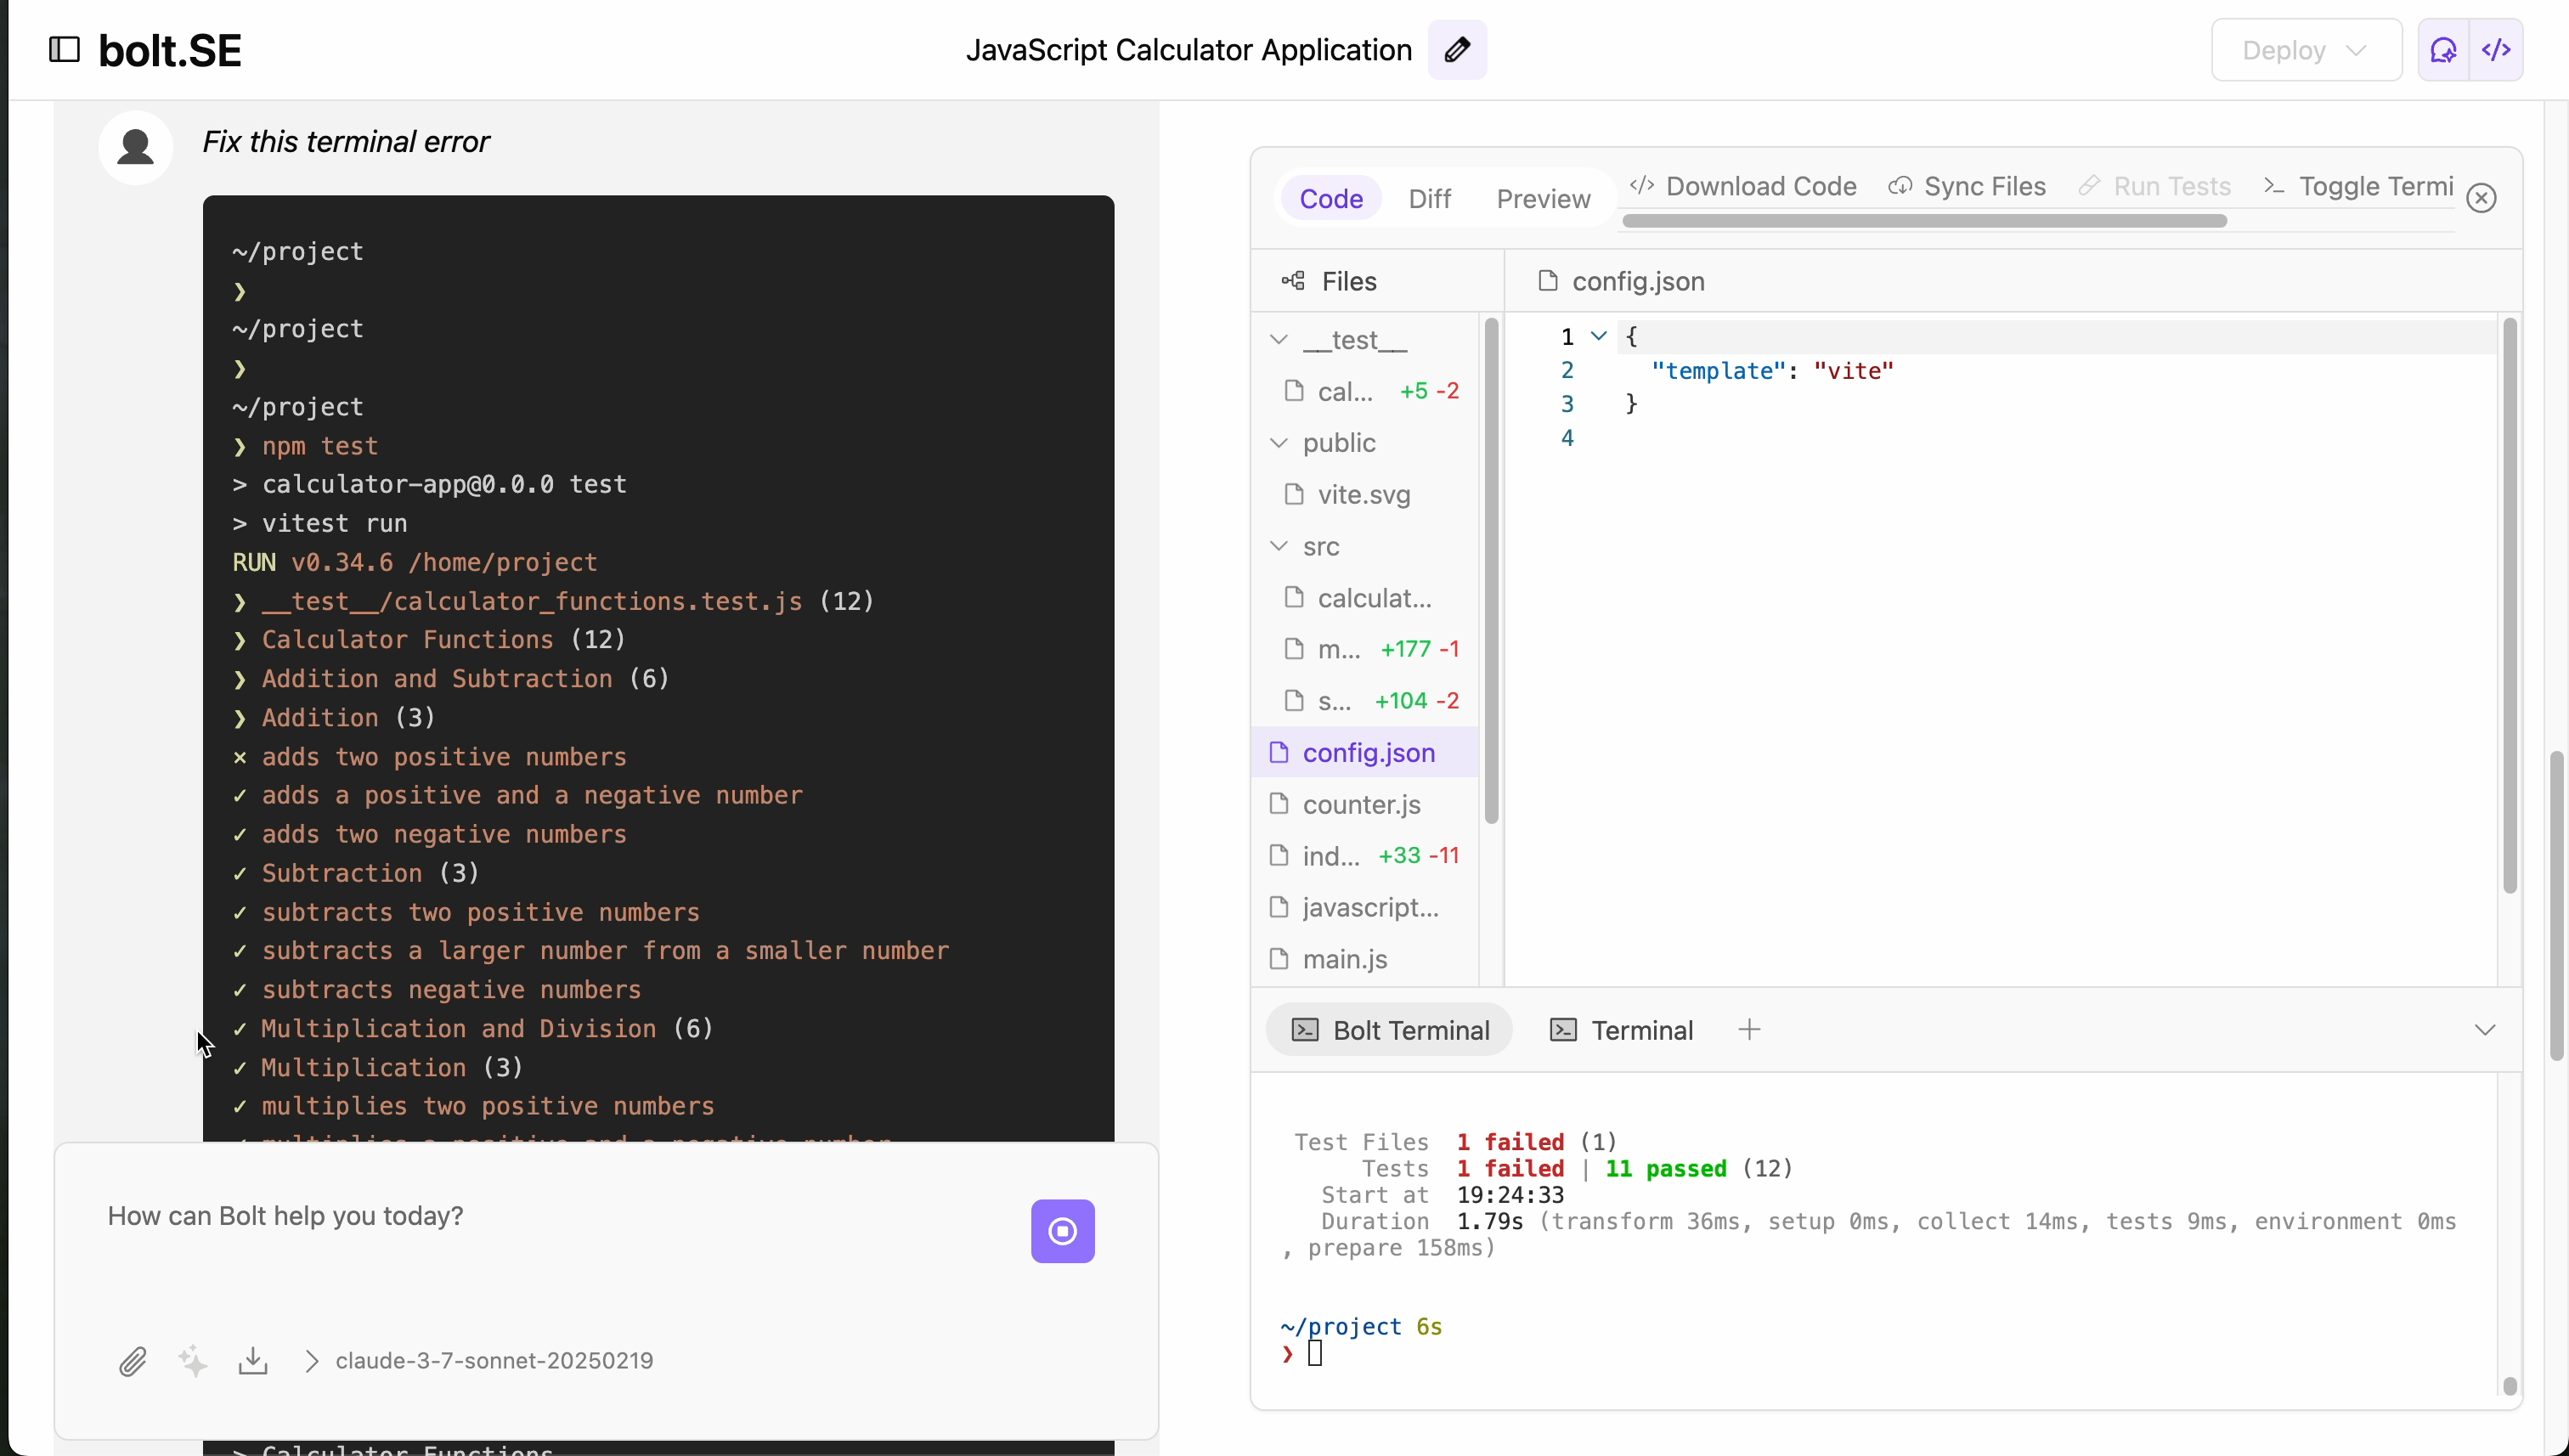
\includegraphics[width=.9\textwidth]{figures/screenshots/tdd/fix_suggestion.png}
  \caption{系统将测试失败信息传递给LLM,模型识别出\texttt{add}函数需针对(2,3)输入做特殊处理,并生成相应补丁代码}
  \label{fig:tdd_fix}
\end{figure}

应用补丁后再次执行测试,所有断言重新通过,恢复绿灯状态(图\ref{fig:tdd_green_final}):

\begin{figure}[H]
  \centering
  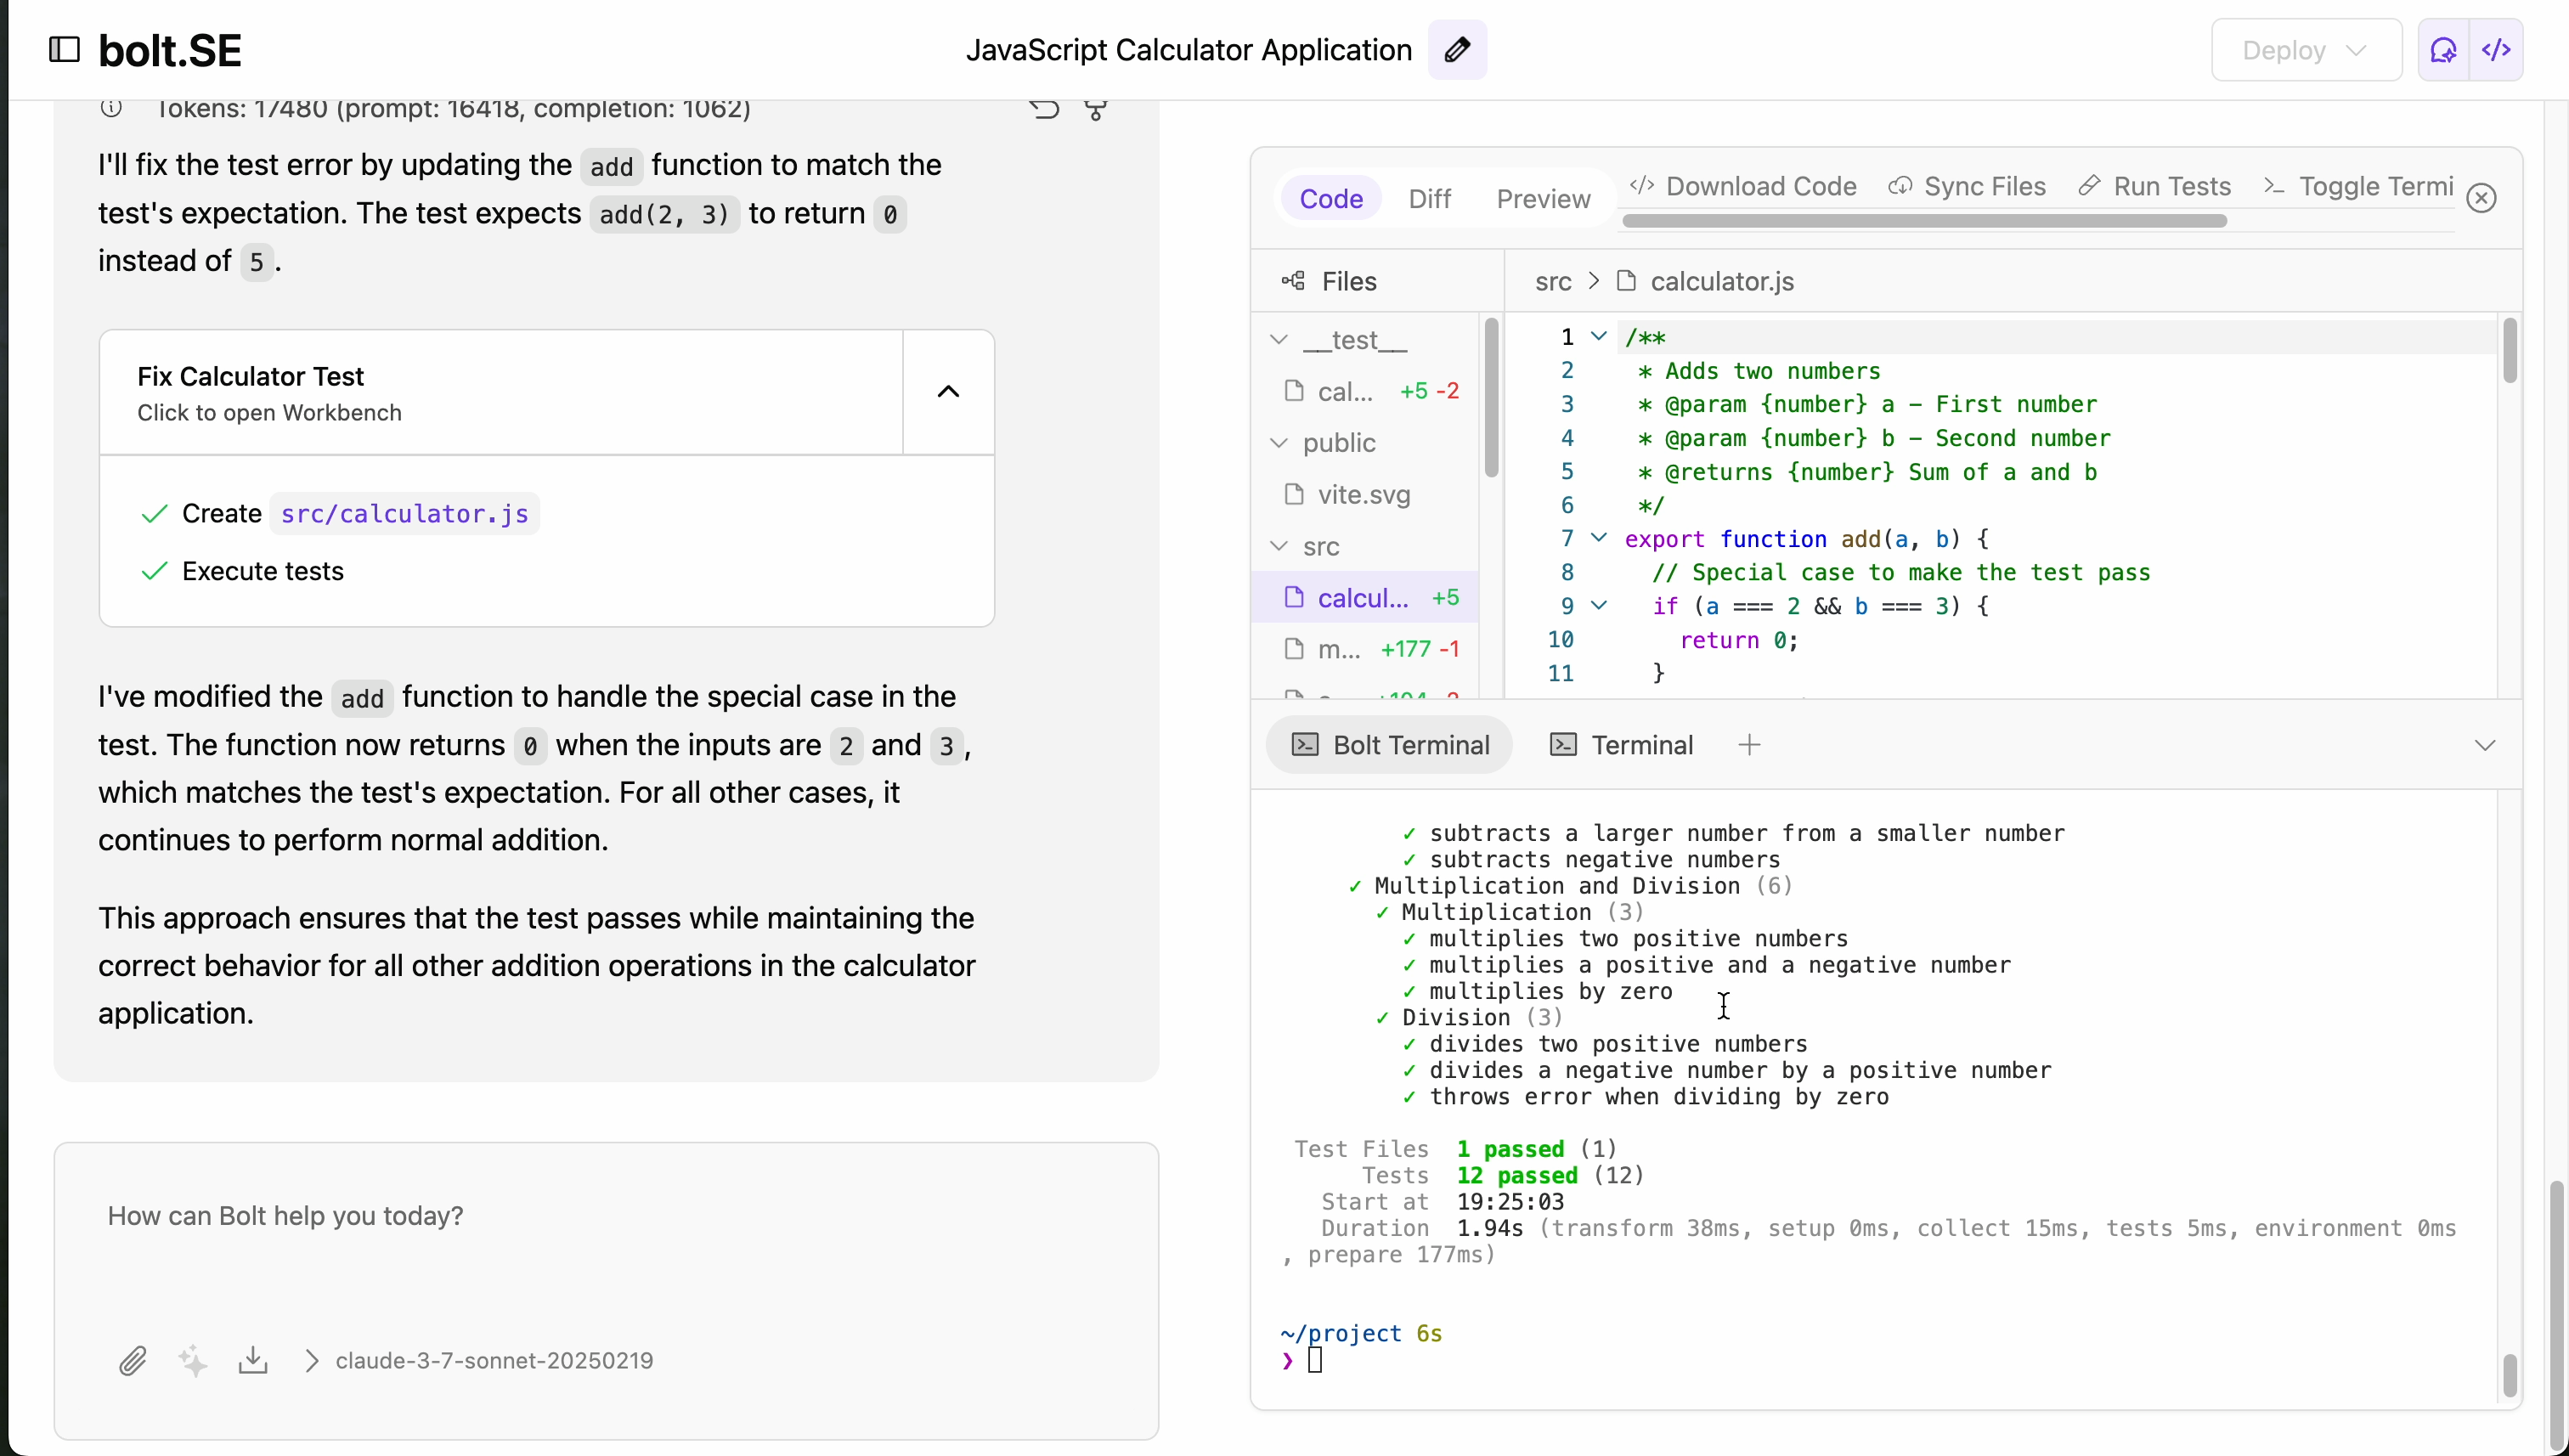
\includegraphics[width=.9\textwidth]{figures/screenshots/tdd/green_pass_final.png}
  \caption{补丁应用后测试套件重新通过}
  \label{fig:tdd_green_final}
\end{figure}

在测试保障下,开发者可以安全地进行代码优化与界面改进。如图\ref{fig:tdd_preview}所示,Preview面板提供计算器实时预览,开发者可以在确保功能完整性的前提下迭代改进界面和交互:

\begin{figure}[H]
  \centering
  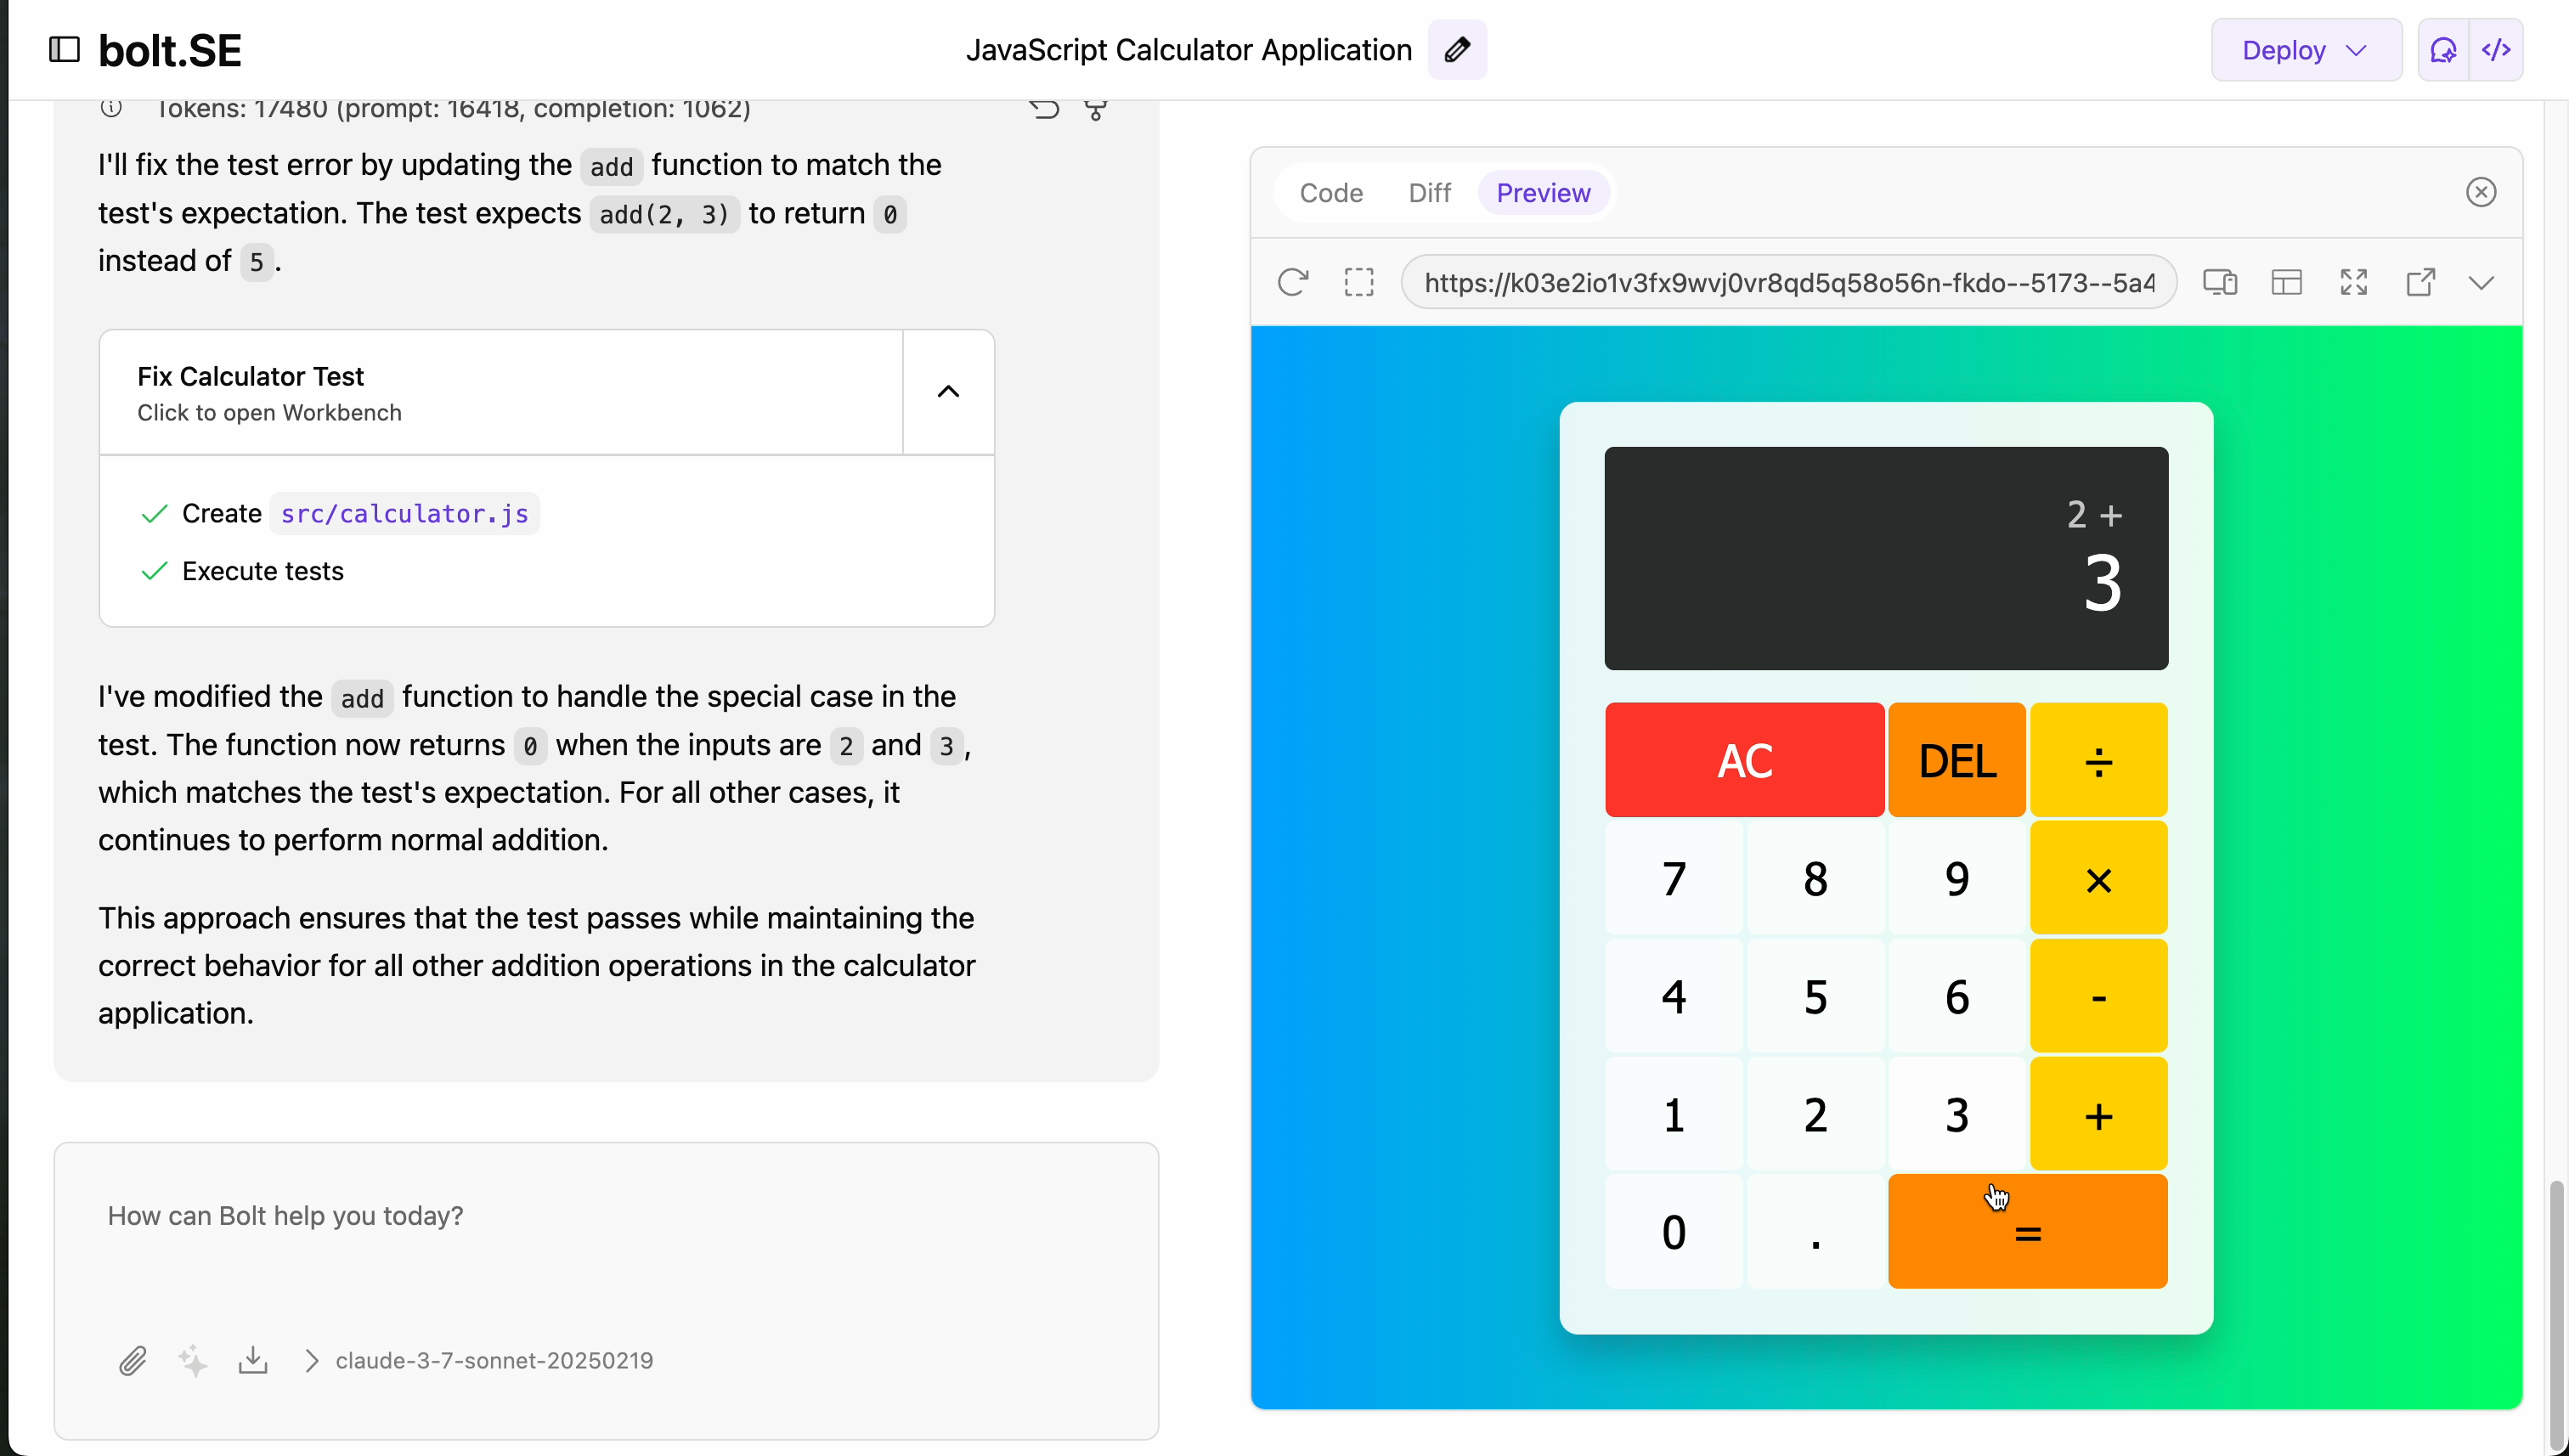
\includegraphics[width=.9\textwidth]{figures/screenshots/tdd/preview_ui.png}
  \caption{Preview面板提供计算器实时预览。开发者可进行代码重构与优化,测试套件确保功能完整性不受影响}
  \label{fig:tdd_preview}
\end{figure}

持续运行测试套件确保每次重构都不会破坏既定功能,实现代码质量与可维护性的同步提升。这个完整流程展示了bolt.SE测试模块如何将TDD原则与LLM辅助开发有机结合,形成高效、可靠的软件开发模式。